%%
%% This is file `sample-authordraft.tex',
%% generated with the docstrip utility.
%%
%% The original source files were:
%% v
%% samples.dtx  (with options: `authordraft')
%% 
%% IMPORTANT NOTICE:
%% 
%% For the copyright see the source file.
%% 
%% Any modified versions of this file must be renamed
%% with new filenames distinct from sample-authordraft.tex.
%% 
%% For distribution of the original source see the terms
%% for copying and modification in the file samples.dtx.
%% 
%% This generated file may be distributed as long as the
%% original source files, as listed above, are part of the
%% same distribution. (The sources need not necessarily be
%% in the same archive or directory.)
%%
%% The first command in your LaTeX source must be the \documentclass command. 

% \documentclass[sigconf,authordraft]{acmart}
\documentclass[sigconf,nonacm]{acmart}

\usepackage[portuges]{babel}

\usepackage{hyperref}
\hypersetup{
    colorlinks=true,
    linkcolor=blue,
    filecolor=magenta,
    urlcolor=cyan,
}

\urlstyle{same}

%%
%% \BibTeX command to typeset BibTeX logo in the docs
\AtBeginDocument{%
  \providecommand\BibTeX{{%
    \normalfont B\kern-0.5em{\scshape i\kern-0.25em b}\kern-0.8em\TeX}}}

%% Rights management information.  This information is sent to you
%% when you complete the rights form.  These commands have SAMPLE
%% values in them; it is your responsibility as an author to replace
%% the commands and values with those provided to you when you
%% complete the rights form.
\setcopyright{acmcopyright}
\copyrightyear{2018}
\acmYear{2018}
\acmDOI{10.1145/1122445.1122456}

%% These commands are for a PROCEEDINGS abstract or paper.
\acmConference[Woodstock '18]{Woodstock '18: ACM Symposium on Neural
  Gaze Detection}{June 03--05, 2018}{Woodstock, NY}
\acmBooktitle{Estratégia para os Dados Abertos}
%\acmISBN{978-1-4503-XXXX-X/18/06}


%%
%% Submission ID.
%% Use this when submitting an article to a sponsored event. You'll
%% receive a unique submission ID from the organizers
%% of the event, and this ID should be used as the parameter to this command.
%%\acmSubmissionID{123-A56-BU3}

%%
%% The majority of ACM publications use numbered citations and
%% references.  The command \citestyle{authoryear} switches to the
%% "author year" style.
%%
%% If you are preparing content for an event
%% sponsored by ACM SIGGRAPH, you must use the "author year" style of
%% citations and references.
%% Uncommenting
%% the next command will enable that style.
%%\citestyle{acmauthoryear}

%%
%% end of the preamble, start of the body of the document source.
\begin{document}

%%
%% The "title" command has an optional parameter,
%% allowing the author to define a "short title" to be used in page headers.
\title{Repositórios de Dados: Objetivos, Funcionalidades e Alternativas}

%%
%% The "author" command and its associated commands are used to define
%% the authors and their affiliations.
%% Of note is the shared affiliation of the first two authors, and the
%% "authornote" and "authornotemark" commands
%% used to denote shared contribution to the research.
\author{João Rocha da Silva}
\authornote{Investigador no INESC TEC e Professor Auxiliar Convidado na Faculdade de Engenharia da Universidade do Porto}
\email{joaorosilva@gmail.com}
\orcid{0000-0001-9659-6256}
\affiliation{%
  \institution{INESC TEC / Faculdade de Engenharia da Universidade do Porto}
  \streetaddress{Campus da Faculdade de Engenharia da Universidade do Porto, Rua Dr. Roberto Frias}
  \city{Porto}
  \state{Portugal}
  \postcode{4200-465}
}

%%
%% By default, the full list of authors will be used in the page
%% headers. Often, this list is too long, and will overlap
%% other information printed in the page headers. This command allows
%% the author to define a more concise list
%% of authors' names for this purpose.
\renewcommand{\shortauthors}{João Rocha da Silva}

%%
%% The abstract is a short summary of the work to be presented in the
%% article.
\begin{abstract}
    Os repositórios de dados de investigação são cada vez mais uma peça essencial para o processo científico. Não só fomentam a reprodutibilidade das conclusões publicadas nos artigos científicos como assumem um papel crucial na atribuição de crédito aos criadores de dados, pois expôem ao público um trabalho de recolha, processamento e anotação que tanto tem de dispensioso como por vezes de invisível.
    A escolha de um software para suportar um repositório de dados deve ser guiada pelas necessidades das principais partes interessadas. Assim sendo, neste artigo discutem-se as principais funcionalidades desejáveis num repositório de dados, tanto do ponto de vista técnico (software e infraestrutura) como do ponto de vista político, nomeadamente no que diz respeito às garantias e compromissos a assumir pelas instituições que os alojam no sentido de permitir a sua certificação de acordo com a estratégia da European Open Science Cloud.
\end{abstract}

%%
%% Keywords. The author(s) should pick words that accurately describe
%% the work being presented. Separate the keywords with commas.
\keywords{repositorios de dados, ciência aberta, e-Science, Estratégia para os Dados Abertos, Fundação para a Ciência e Tecnologia}

%% A "teaser" image appears between the author and affiliation
%% information and the body of the document, and typically spans the
%% page.
% \begin{teaserfigure}
%   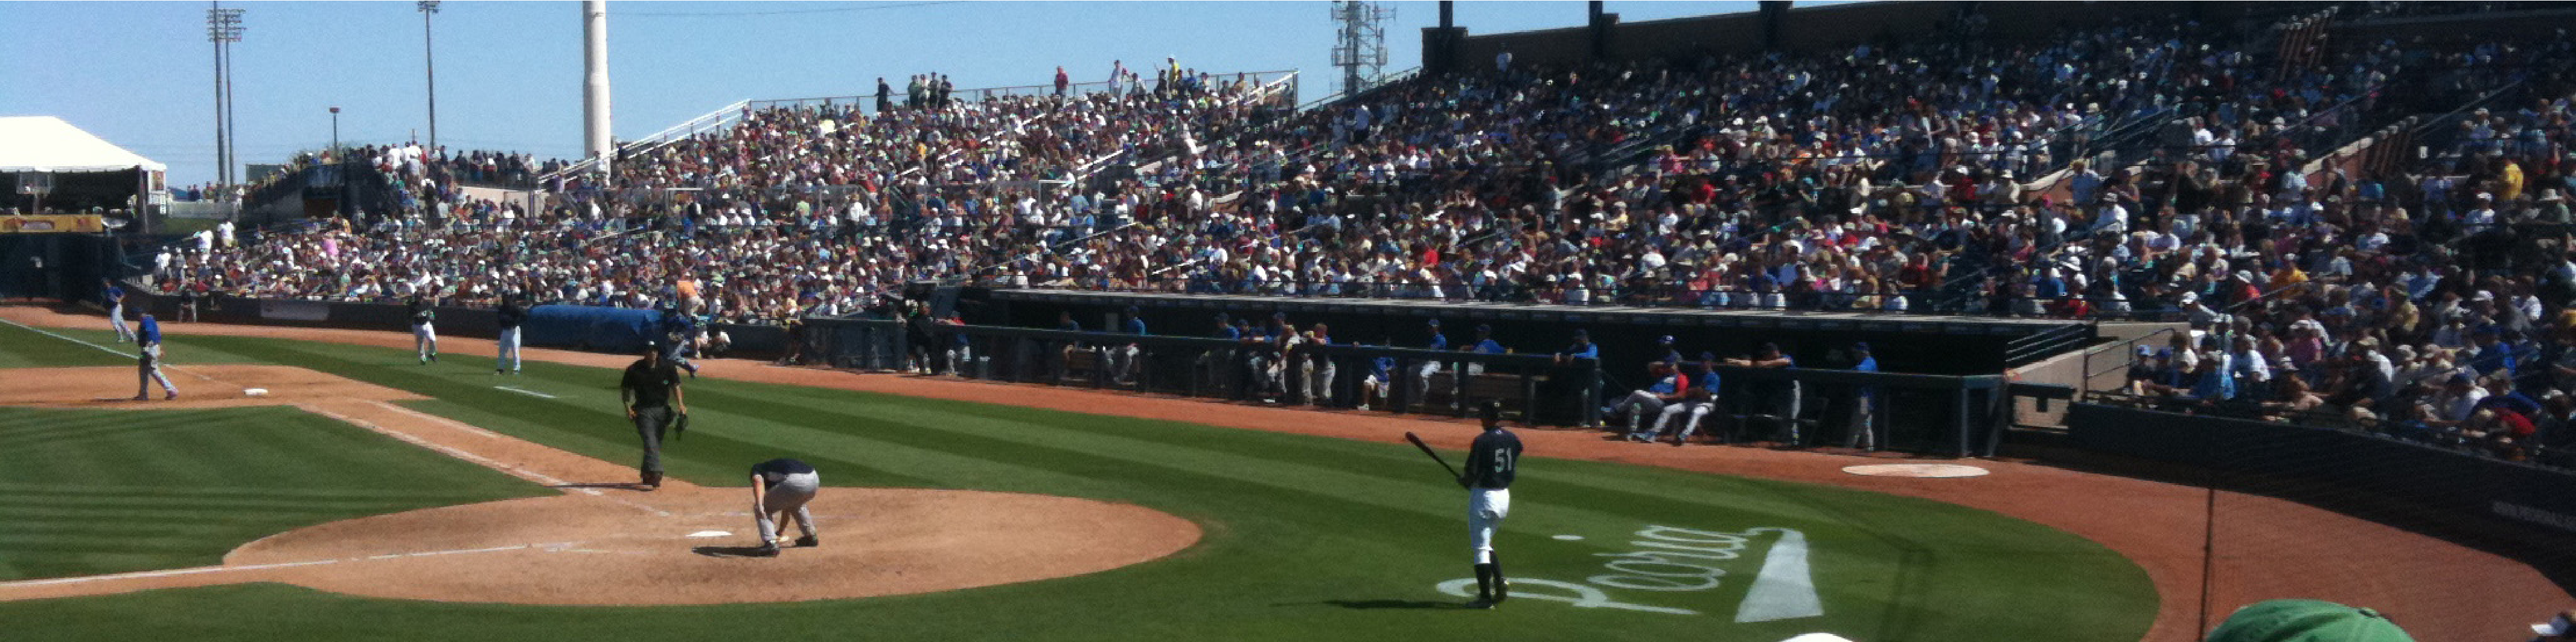
\includegraphics[width=\textwidth]{sampleteaser}
%   \caption{Seattle Mariners at Spring Training, 2010.}
%   \Description{Enjoying the baseball game from the third-base
%   seats. Ichiro Suzuki preparing to bat.} 
%   \label{fig:teaser}
% \end{teaserfigure}

%%
%% This command processes the author and affiliation and title
%% information and builds the first part of the formatted document.
\maketitle

\section{Introdução}

Os princípios FAIR para a gestão de dados de investigação especificam que os dados devem ser Findable (encontráveis), Accessible (acessíveis), Interoperable (interoeráveis) and Reusable (reutilizáveis)~\cite{wilkinson2016fair}. 

Recentemente, um grupo de peritos da Comissão Europeia debruçou-se sobre o problema dos dados FAIR, tendo concluído que os componentes essenciais de um ecossistema FAIR são: políticas, planos de gestão de dados (DMP), identificadores, normas e repositórios~\cite{hodson2018turning}. 


Neste artigo serão abordados alguns destes tópicos.

\section{O papel do repositório na aplicação dos princípios FAIR}

Os princípios FAIR são linhas orientadoras para a melhoria dos processos de gestão de dados, abarcando portanto aspetos bastante mais genéricos do que a tecnologia que suporta um repositório de dados. Contudo, dado que este artigo é bastante focado na tecnologia, utilizaremos os princípios FAIR como guiões orientadores para elencar algumas das funcionalidades relevantes de um repositório de dados. 

O primeiro dos princípios FAIR diz que os dados devem ser \emph{Findable}, ou seja, devem ser fáceis de descobrir, tanto por humanos como por máquinas. Para tal, devem incluir (F1) um identificador global único e persistente, (F2) possuir metadados ricos, que por sua vez (F3) devem incluir claramente o identificador dos recursos que descrevem. O quarto e último aspeto, (F4), especifica que os tanto dados como metadados devem estar registados em recursos pesquisáveis. 

De forma a facilitar a satisfação destes requisitos, uma plataforma de repositório deverá começar por proporcionar integração programática com um fornecedor de identificadores persistentes como por exemplo DOI\footnote{Digital Object Identifier} ou handle\footnote{\url{http://www.handle.net/}}. A vantagem para os gestores de repositório é a possibilidade de atribuir identificadores automaticamente aos conjunto de dados disponibilizados. Um identificador persistente funciona, em palavras simples, como um atalho para um programa num computador. Não é uma cópia do conjunto de dados, mas sim apenas um apontador para o local onde esse conjunto de dados está publicado (tipicamente, um repositório). Sendo assim, deve poder ser \emph{de-referenciado}, ou seja, deve ser possível obter o conjunto de dados a partir do seu identificador. Para um ser humano, tal operação pode consistir apenas num simples clique numa ligação apresentada no seu navegador Web; para uma máquina, contudo, pode ser um pedido de rede à plataforma que gere os identificadores. Em ambos os casos, a entidade solicita o recurso por detrás daquele identificador; no caso do humano, a resposta será em HTML, código que o seu navegador pode interpretar de forma a construir  uma página web legível para humanos. Para uma máquina, o formato devolvido poderá ser, por exemplo XML ou RDF (formatos de representação de informaçºao que as máquinas podem interpretar). 

No caso do repositório de dados do INESC TEC\footnote{Ligação: \url{https://rdm.inesctec.pt}}, a FCT negociou um contrato para a aquisição de pacotes de identificadores em colaboração com a DataCite\footnote{Ligação: \url{https://datacite.org/}}, que permitiu ao repositório emitir DOI para os conjuntos de dados despositados. 

Para satisfazer os requisitos F2 e F3 é necessário que os registos de metadados associados a cada conjunto de dados obedeçam a um esquema normalizado, como é o caso do DataCite Schema\footnote{Ligação: \url{https://schema.datacite.org/meta/kernel-4.3/}}. Uma grande vantagem do uso de um esquema de metadados em conjunção com a atribuição de um DOI é que cada identificador ficará associado a uma ficha de metadados no momento da \emph{cunhagem} do DOI. Tipicamente, as plataformas de emissão de identificadores não permitem sequer a sua cunhagem sem o preenchimento dessa ficha de metadados. Esta ficha ficará então guardada na plataforma emissora do DOI, e mesmo que o conjunto de dados deixe de estar disponível no repositório, a ficha continuará disponivel para consulta na plataforma fornecedora do identificador (satisfazendo o requisito A2, descrito a seguir).

O segundo princípio FAIR impõe que os dados sejam \emph{Accessible}, pois tanto dados como metadados devem ser acessíveis através através de identificadores, através de protocolos de comunicações normalizados (A1). Este ponto requer que o protocolo seja aberto, livre e universalmente implementável (A1.1), e que inclua procedimentos de autenticação e autorização, quando necessário (A1.2). O segundo requisito para assegurar a acessibilidade (A2) é que os metadados devem permanecer acessíveis, mesmo quando os dados deixam de o estar.

Para satisfazer o requisito A1, um repositório deverá suportar o processo de des-referenciação de identificadores persistentes, quer por máquinas quer por seres humanos. Quando se fala de protocolos de comunicações normalizados, falamos quase sempre do protocolo HTTP. Este é talvez o protocolo mais usado na web para transferência de informação, e satisfaz o requisito A1. Ele inclui dois mecanismos relevantes para a satisfação do requisito A1.1, chamados \emph{Content Negotiation}\footnote{Ligação: \url{https://www.w3.org/Protocols/rfc2616/rfc2616-sec12.html}}, Authorization \footnote{Ligação: \url{https://www.w3.org/Protocols/HTTP/1.0/draft-ietf-http-spec.html\#Authorization}} e Access Authentication\footnote{Ligação: \url{https://www.w3.org/Protocols/HTTP/1.0/draft-ietf-http-spec.html\#BasicAA}}. 

De uma forma muito breve, este mecanismo permite a um cliente (pode ser um navegador web ou um programa de computador) solicitar ao servidor (máquina que disponibiliza o registo de metadados de um determinado conjunto de dados) que envie a informação determinado formato, ao escrever esse pedido no cabeçalho do pedido HTTP (que pode ser visto como a secção ``Destinatário'' de um envelope). Ao especificar que pretende HTML, um navegador irá obter o código necessário para apresentar os dados sobre o conjunto de dados a um ser humano; se uma máquina solicitar XML ou RDF, irá obter um documento que é muito mais difícil de ler por parte de um ser humano, mas que a máquina interpreta corretamente. A beleza deste sistema de negociação é que permite obter essas diferentes representações a partir de um mesmo identificador, mudando apenas o cabeçalho da mensagem.

Apesar da autenticação básica oferecida pelo protocolo HTTP ser suficiente para satisfazer requisito A1.1, existem protocolos alternativos que podem ser adoptados caso hajam outros requisitos relevantes para a instituição que implementa um repositório de dados. Listam-se alguns protocolos abertos que podem ser relevantes neste cenário:

\begin{itemize}
  \item \textbf{Autenticação federada}: O protocolo Shibboleth\footnote{Ligação: \url{https://www.shibboleth.net/index/}} é bastante usado nas instituições de ensino superior portuguesas para controlar o acesso a multiplos recursos através do portal de autenticação federada oferecido pela FCCN. Um repositório institucional deverá registar-se junto do Identity Provider relevante para permitir aos utilizadores autenticar-se com as mesmas credenciais que usam para aceder aos restantes recursos da sua instituição.
  \item \textbf{Autenticação delegada via outros providers}: O protocolo OAuth 2.0\footnote{Ligação: \url{https://oauth.net/2/}} permite aos utilizadores autenticar-se com as mesmas credenciais que utilizam em outros serviços como o ORCID\footnote{Ligação: \url{https://members.orcid.org/api/oauth2}}, que pode ser útil para assegurar a autenticidade de auto-depósitos ou modificações feitas aos metadados pelos próprios criadores dos mesmos. Desta forma, podemos garantir que se uma determinada operação é realizada por alguém, se esse alguém se tiver autenticado com sucesso junto do ORCID, por exemplo. Este mecanismo foi implementado na plataforma de gestão de dados Dendro, para agilizar o registo de novos utilizadores e a sua autenticação. Desta forma, o identificador ORCID de cada utilizador ficará associado ao seu perfil, e indiretamente às operações efetuadas por esse utilizador no repositório.
\end{itemize}


O terceiro princípio FAIR diz que a gestão de dados deve ser \emph{Interoperable}. Isto deve-se ao facto dos dados precisarem frequentemente de ser integrados com outros dados, e como tal têm que ser facilmente integráveis em fluxos de trabalho de processamento. Só assim podem ser facilmente armazenados e analisados de forma interoperável. Para assegurar a interoperabilidade, tanto dados como metadados devem (I1) usar uma linguagem formal, acessível e largamente aplicada para representação de conhecimento, (I2) devem usar vocabulários que, por sua vez, seguem os princípios FAIR, e (I3) devem incluir referências qualificadas para outros dados e metadados.

Talvez o princípio mais difícil de assegurar, a interoperabilidade implica a representação da informação constante no repositório em formatos que permitam a interpretação por sistemas externos. Isto quer dizer que os dados devem ser representados não só em formatos amigáveis como largamente suportados pelas bibliotecas de manipulação de dados mais usadas e disponíveis em código aberto. Para os dados, por exemplo, devem ser adotados os formatos livres de dependências e largamente suportados, como por exemplo XML, CSV ou TSV, em detrimento de formatos binários ou proprietários. Para os metadados, devem ser representados com recurso a standards bem definidos na comunidade, sejam eles formalizados como esquemas XML, ou ontologias no caso do repositório disponibilizar os registos de metadados como Linked Data. 

Alguns exemplos destes esquemas incluem o amplamente utilizado Dublin Core ou o schema.org, um esquema de metadados para a web que reuniu a colaboração das principais tecnológicas (Google, Microsoft, Yahoo e Yandex)\footnote{Ligação: \url{https://schema.org/}}, que possam tanto ser formalizados como esquema XML como sob a forma de ontologias. Sejam qual forem os vocabulários seleccionados, devem eles próprios seguir os princípios FAIR, estando portando livremente acessíveis e serem devidamente documentados. 

Por último, a interoperabilidade também diz respeito à inclusão de referencias para recursos relacionados. Por último, deverão ser incluídas nos registos de metadados de cada conjunto de dados referências para materiais relacionados. Exemplos de materiais relacionados incluem por exemplo um documento de dissertação ou tese, artigos resultantes da produção dos conjuntos em questão. Os esquemas ou ontologias utilizadas para a descrição devem portanto incluir descritores que permitam essas referências, como é o exemplo do descritor \texttt{references} do Dublin Core\footnote{Ligação: \url{https://www.dublincore.org/specifications/dublin-core/dcmi-terms/terms/references/}} ou o descritor \texttt{citation} do schema.org\footnote{\url{https://schema.org/citation}}.

O quarto e último dos princípios defende que os dados devem ser \textit{Reusable}, pois o objetivo final dos princípios FAIR é fomentar a sua reutilização. Para serem Reutilizáveis, tanto dados como metadados devem (R1) ser descritos com uma grande variedade de atributos corretos e relevantes. Este princípio subdivide-se em três: (R1.1) devem ser publicados com uma licença de utilização clara e acessível, (R1.2) devem estar associados a informação de proveniência detalhada, sendo que esses dados e metadados devem satisfazer as normas relevantes de cada domínio (R1.3).

As licenças a escolher (recomendação R1.1) ficam ao critério da instituição de investigação e do criador dos dados. Contudo, para a disponibilização de dados de investigação em regime de \emph{Open Data} é desejável a adoção de licenças que permitam a reutilização dos dados e metadados com o mínimo de restrições. Por forma a proporcuinar a outros a liberdade de reutilizar os dados para produzir trabalhos derivados e ao mesmo tempo assegurar a atribuição de crédito aos autores, as licenças Creative Commons (nomeadamente a CC BY-4.0)\footnote{Ligação: \url{https://creativecommons.org/licenses/by/4.0/}} é uma boa candidata na maioria dos casos de conjuntos de dados produzidos por projetos financiados por entidades públicas. Grande parte dos investigadores podem, no entanto, sentir dificuldades no momento da escolha da licença mais adequada para os conjuntos de dados que desejam publicar. É nesta altura que uma plataforma de repositório pode complementar o trabalho dos curadores, ao fornecer uma lista das licenças mais comuns, e ao mesmo tempo proporcionar tanto descrições curtas, claras e sucintas de cada licença, e ao mesmo tempo oferecer uma ligação rápida para a licença completa em linguagem jurídico-legal. 

A recomendação R1.2 refere a necessidade de manter um historial que permita estabelecer a proveniência de um conjunto de dados. Enquanto que é relativamente simples manter um historial de modificações dentro de uma plataforma de repositório, o desafio é maior quando se considera que um conjunto de dados pode ser derivado de outro, tendo este último o seu próprio historial de modificações. Mais uma vez existe uma clara vantagem em usar Linked Data como formato de exposição de metadados (incluindo a proveniência) neste cenário. Para tal, é necessário que os repositórios de dados ofereçam um histórico de modificações em Linked Data que obedeça a ontologias como a PROV-O\cite{lebo2013prov} (mais normativa pois é recomendação W3C) ou a PAV~\cite{ciccarese2013pav} (uma alternativa mais simples, também apelidada de \emph{lightweight ontology}). Desta forma, quando uma terceira máquina des-referenciar o conjunto de dados derivado será também interrogado o repositório onde se encontra o conjunto de dados original, e assim sucessivamente se ele próprio também for um conjunto de dados derivado. Desta forma, torna-se transparente e automática a recuperação de todos os dados relativos ao historial de modificações e versões de um conjunto de dados, sem necessidade de indexar todos os recursos e sem que haja lugar à intervenção humana.

É bastante claro que domínios de investigação distintos poderão gerar conjuntos de dados muito diferentes também. Como tal, o processo de descrição dos mesmos deve também ser adaptado. Satisfazer a recomendação R1.3, que preconiza que os dados e metadados devem obedecer às normas vigentes em cada domínio requer suporte por parte do software de repositório, que deve ser flexível ao ponto de permitir a parametrização de múltiplos esquemas de metadados para distintos domínios. Deverá também permitir a escolha e combinação de múltiplos descritores (genéricos e específicos do domínio do conjunto de dados em depósito) aquando do preenchimento do registo de metadados, sejam esses descritores genéricos ou específicos de domínio. É preciso também não esquecer o trabalho fundamental dos curadores no apoio institucional aos seus investigadores, pois a escolha dos descritores mais adequados a cada conjunto de dados

\section{Visão geral de funcionalidades}

Existem diferentes alternativas para a montagem de um repositório de dados. Uma análise comparativa produzida pelo projeto Dataverse\footnote{Ligação:  \url{https://dataverse.org/blog/comparative-review-various-data-repositories}} apresenta uma comparação das principais plataformas de repositórios de dados, tendo em conta três grupos de facetas: Funcionalidades de Software, Controlo/Organização e Conteúdo. 

Uma outra comparação~\cite{amorimComparison2017} discute em mais profundidade algumas características técnicas de diversas plataformas. Esta análise foca-se apenas nas alternativas disponíveis em regime de código aberto e instaláveis localmente, para poder retirar conclusões relativamente ao modelo de dados por detrás de cada solução de software. 

Há muitas formas de categorizar estas plataformas, mas existem duas categorias principais: serviços ``chave-na-mão'', em que todas as necessidades do serviço (alojamento, manutenção, assistência técnica, curadoria ou atribuição de identificadores) faz parte de um pacote oferecido às instituições interessadas em partilhar conjuntos de dados. Em alternativa, apresentam-se as soluções alojadas localmente. Estas diferem em relação às suas alternativas ``chave-na-mão'' na medida em que exigem instalação e manutenção por parte de uma equipa de IT interna à organização. O trabalho de curadoria na plataforma também tem que ser levado a cabo inteiramente pelos elementos da organização e geralmente não existe nenhuma obrigação de assistência por parte dos desenvolvedores do software. Contudo, nos projetos de software open-source existe normalmente um fórum público onde os utilizadores podem propor melhorias ao software e reportar \textit{bugs}.


Tão importante como comparar funcionalidades oferecidas pelas plataformas é estudar quais funcionalidades são mais valorizadas pelos utilizadores destas plataformas. Para responder a esta questão, o Grupo de Interesse das Plataformas de Gestão de Dados de Investigação (RPRD IG) da Research Data Alliance (RDA) compilou uma Matriz de Casos de Uso e Requisitos Funcionais para as Plataformas de Gestão de Dados de Investigação. Esta matriz resultou de um inquérito a 11 grupos que apresentaram os seus casos de uso para repositórios de dados de investigação. Cada um destes grupos classificou a importância de 26 requisitos vulgarmente associados a um repositório de dados. No final, foi atribuída uma pontuação a cada um dos requisitos funcionais, com base na importância que a totalidade dos grupos lhe atribuiu no contexto do seu caso de uso.

Analisando a matriz de requisitos funcionais, é possível ver que %TODO

\section{Certificação}

Para além dos princípios FAIR, que se apresentam como linhas gerais para aquilo que um processo de gestão de dados deve proporcionar, surgiram recentemente os princípios TRUST~\cite{TRUSTprinciples}. Estes focam-se no problema da confiança nas infraestruturas, organizações e qualidade dos dados de investigação. Estes princípios oferecem, de acordo com os autores, uma \emph{framework} de discussão para ajudar a melhorar a confiança de todas as partes interessadas no processo de gestão de dados. Estas partes interessadas vão desde os próprios investigadores, passando pelas instituições académicas ou de ciência que os acolhem, as entidades financiadoras, entre outros~\cite{DCC_stakeholders}. 

De acordo com o Guião Estratégico de Implementação (GEI) da EOSC (European Open Science Cloud), a certificação de repositórios de dados é uma parte essencial na visão a longo prazo da Comissão Europeia. 

Já de um ponto de vista mais económico e de soberania dos dados, a certificação de repositórios assumirá um papel cada vez mais importante no funcionamento de uma instituição académica ou de investigação. Existem diversas razões, de entre as quais se destaca o crescente número de entidades financiadoras e publicações de renome que exigem a disponibilização dos dados-base e do código-fonte que sustenta as publicações. Neste cenário, a qualidade dos repositórios onde tais recursos são disponibilizados terá necessariamente que ser elevada. Desta forma, a certificação tornar-se-à assim uma pedra fundamental no suporte aos projetos de investigação, pois as instituições terão que assegurar aos seus investigadores a satisfação dos presentes e futuros requisitos de financiadores aquando da escrita dos planos de gestão de dados a anexar às propostas de financiamento.

Essas instituições terão então duas opções para garantir os requisitos : ou embarcam num processo de certificação dos seus próprios repositórios institucionais, ou subcontratam o processo de depósito e curadoria de dados a um repositório certificado. 

\section{Automatização da gestão de dados}

Qualquer processo de gestão de dados de investigação deve começar com o desenho de um Plano de Gestão de Dados (ou DMP, do inglês Data Management Plan). Um DMP é um documento tipicamente escrito e aprovado antes do início de um projeto de investigação. Em alguns casos, é já requisito obrigatório em chamadas de propostas de projetos de investigação suportados por fundos públicos~\cite{Foundation2011}) e que especifica todos os aspetos relacionados com a gestão dos dados produzidos ao longo do projeto~\cite{}.  

Entre outros aspetos, que dados serão produzidos no contexto de um projeto, que metadados serão anexados aos dados publicados, onde eles irão ficar disponíveis após o fim do projeto, entre outros pontos. No Reino Unido, o Digital Curation Centre disponibiliza tanto um guião~\cite{jones_dmp} para a escrita deste tipo de documentos como uma ferramenta online, o DMP Online~\footnote{\url{Ligação: https://dmponline.dcc.ac.uk}}, que assiste os investigadores e curadores na elaboração dos seus DMP, assistidos por uma base de dados de templates de DMP aceites por diferentes entidades financiadoras.

Com a grande quantidade de dados de investigação gerada diariamente surge a necessidade de acompanhar e monitorizar a implementação de DMP, mas de forma automática. Três exemplos simples de operações frequentes, repetitivas e facilmente automatizáveis são: 

\begin{itemize}
    \item Simples verificação da disponibilidade dos dados depositados
    \item Controlo de qualidade dos metadados associados aos conjuntos de dados acabados
    \item Verificação das licenças associadas aos conjuntos de dados
\end{itemize}

Para lidar com estas operações e outras de forma mais automática surgiram os chamados DMP Accionáveis por Máquina (maDMP, do inglês \textit{Machine-Actionable DMP}). Desta forma é possível assim libertar os curadores de dados para outras operações menos automatizáveis, como o suporte direto aos investigadores ou atividades de formação.

Como preconizado pelos autores das 10 regras para maDMP~\cite{miksa_tomasz_2018_1172673}, deve ser possível aos sistemas informáticos levar a cabo ações em nome das partes interessadas no processo de gestão de dados de investigação. Operações dadas como exemplo incluem a recolha automática de informação administrativa relevante para anotação dos recursos produzidos. Exemplos dessa informação incluem, por exemplo, as recuperação de referências aos financiadores dos projetos, os currículos dos autores dos conjuntos de dados assim como as informações corretas das instituições de acolhimento dos investigadores. 

Esta necessidade de suporte a automação e integração tem implicações vastas do ponto de vista do desenho e funcionalidades de um repositório de dados, na medida em que a solução deve disponibilizar uma API (\textit{Application Programming Interface}) completa e bem documentada, de forma a permitir a sistemas externos executar estas operações sem a necessidade de intervenção humana.

\subsection{O papel da interoperabilidade na descoberta de conjuntos de dados}

Ao mesmo tempo, a integração com diretórios de dados deve ser transparente e assente em protocolos de interoperabilidade standard. Estes agregadores são portais que indexam o conteúdo dos repositórios para facilitar a pesquisa e descoberta de recursos neles contidos. Exemplos destes agregadores são, por exemplo, o portal re3data da DataCite~\footnote{Ligação: \url{https://www.re3data.org/}} ou o Dataset Search da Google\footnote{Ligação: \url{https://datasetsearch.research.google.com/}}.

Para facilitar a indexação dos conteúdos dos repositórios, estes implementam suporte ao protocolo OAI-PMH (Open Access Initiative Protocol for Metadata Harvesting). Este protocolo expõe os metadados de todos os registos no repositório de forma paginada, para que seja lida sequencialmente e indexada; contudo, não possibilita a pesquisa e recuperação de registos específicos por termos contidos nos registos de metadados, por exemplo. Para conseguir tal funcionalidade é necessário proceder à inserção de todos os documentos num índice de pesquisa como é o caso do Lucene ou Solr. Uma consequência óbvia é a necessidade de manutenção de cópias dos registos e atualizações periódicas de todo o índice---uma operação lenta e dispendiosa em termos de recursos informáticos, que coloca todo o custo de manutenção do serviço do lado dos clientes.

Uma situação oposta ocorre com a adoção de Dados Ligados (\textit{Linked Data}) na representação de metadados para conjuntos de dados de investigação. Esta representação de dados vem eliminar a necessidade de indexação periódica de conteúdos e melhorar muito a precisão das pesquisas, caso os dados sejam estruturados de acordo com uma ou mais ontologias. Uma ontologia é definida, na Ciência da Informação, como uma \textit{especificação de uma conceptualização}\cite{gruber1995toward}, que permite às máquinas, por exemplo, interpretar o significado dos tipos de entidades representadas num sistema e as relações que se podem estabelecer entre elas.

A representação via Linked Data permite uma maior descentralização da carga de pesquisas sobre os servidores onde os repositórios estão alojados. Reduz também a necessidade de indexação porque é possível correr pesquisas nos próprios servidores sem ter que primeiro indexar todo o seu conteúdo e permite aos clientes do serviço recuperar conjuntos de dados com muito mais precisão do que nos casos em que se usa um índice de pesquisa simples baseado em palavras-chave, pois é possível especificar critérios muito detalhados sob a forma interrogações SPARQL.

A disponibilização de Linked Data por parte dos repositórios tem, contudo, um custo para quem hospeda esses repositórios. As consultas SPARQL são exigentes do ponto de vista computacional e, se um número elevado de utilizadores (máquinas ou humanos) aceder ao website ao mesmo tempo, é fácil afetar os tempos de resposta da infraestrutura. Isto é especialmente relevante quando se considera a funcionalidade de pesquisa federada, onde múltiplos servidores podem ser contactados para conseguir obter os resultados pretendidos por uma única pesquisa iniciada em qualquer dos nós da federação.

O futuro dos repositórios de dados deve passar assim por uma solução híbrida, onde servidores e clientes partilham informação para possibilitar também a partilha do esforço de interrogação e descoberta de dados. Soluções como a Linked Data Fragments\cite{VERBORGH2016184} propõem a combinação de interrogações sobre \textit{endpoints} tradicionais (no servidor do repositório que expõe Dados Ligados) com a interrogação a dados locais a cada cliente, reduzindo assim a carga sobre o servidor.

\subsection{Repositórios como plataformas de computação}

Cada vez mais, o valor de um repositório de dados reside na facilidade de reutilização dos dados nele contidos. Tecnologias recentes como os Research Notebooks e a Containerização permitem tornar os algoritmos mais portáteis portáteis, de forma a poderem ser executados remotamente sobre os dados depositados num repositório. O papel deste torna-se assim muito mais do que o de simples armazenista, indexador e recuperador de pacotes de dados.

É muito comum descobrir conjuntos de dados que, apesar de publicados e devidamente descritos com metadados completos, não são interpretáveis ou reproduzíveis quando um investigador tenta repetir os passos experimentais reportados num artigo de investigação\cite{}. 

Os Research Notebooks são cadernos de laboratório interactivos que encerram em si os dados-base, código de processamento que transforma os dados base em dados processados, e até mesmo visualizações e gráficos gerados na hora com base nos dados e no código do Notebook.

Os Notebooks vêm também possibilitar suportar uma dos maiores mudanças no paradigma de publicação científica dos últimos tempos. A combinação elegante de texto, trechos de código e visualizações apelativas permitiu a criação dos chamados ``Web Journals'' como por exemplo o distill.pub. Estes distinguem-se das publicações convencionais, ao incorporar visualizações interativas no próprio texto dos artigos científicos, fomentando a experimentação através da manipulação de parâmetros de entrada dos algoritmos, produzindo um feedback visual imediato aos leitores. Toda a computação tem, no entanto, que ser executada em tempo real, o que implica a montagem de uma réplica do ambiente de processamento por detrás do portal web que suporta o journal.

Com o problema do empacotamento do processamento e dos dados a ser abordado pelos Notebooks, resta o problema de onde realizar a execução desses algoritmos. Nem todos os conjuntos de dados se prestam a ser transportados pela rede em tempo útil para a execução de um determinado algoritmo, pois em certas disciplinas o seu tamanho pode ascender a centenas de gigabytes ou mesmo terabytes. Assim sendo, é necesário levar a computação até aos dados em vez de ter que transmitir os dados até ao local onde se realiza a computação. Este tipo de computação que ocorre junto dos dados é um paradigma é implementado em portais de computação como o D4Science~\footnote{Ligação: \url{https://www.d4science.org}} ou o EUDAT B2Stage\footnote{Ligação: \url{https://www.eudat.eu/b2stage}}. Com a esperada descentralização e interoperabilidade que se espera dos repositórios de dados defendida pelo GEI da EOSC, espera-se que cada repositório seja capaz de oferecer capacidade de computação local a pequena escala e junto das fontes de dados. Este cenário é mais próximo do \emph{edge computing}, um termo mais vulgarmente associado às aplicações IoT. Por contraponto ao \emph{cloud computing}, onde todos os recursos se encontram na nuvem e os dados têm que ser cuidadosamente aproximados dos nós de computação (mesmo em termos geográficos) para reduzir tráfego na rede, o \emph{edge computing} defende que cada nó da rede deve ter uma pequena mas importante capacidade de computação para executar operações à medida que os dados são produzidos ou atualizados. 

Quando se fala de distribuição de computação e reproducibilidade, surge imediatamente a necessidade de replicar também todo o ambiente de execução no qual essa computação é executada. Sem uma solução de virtualização, isso implica a instalação de um sistema operativo e de todas as dependências relevantes para a execução do código relevante. Este é um processo manual e dispendioso que torna claramente necessário assegurar a portabilidade do ambiente de execução, tornando-o instalável automaticamente em qualquer nó com o mínimo de dependências. 

A containerização é uma tecnologia de virtualização que, quando comparada com as máquinas virtuais convencionais, elimina a necessidade de virtualizar um sistema operativo para executar um determinado programa, substituindo essas dependências por um ambiente de execução (ou \textit{runtime}) próprio. O exemplo mais comum de ambiente de virtualização é o Docker\footnote{Ligação: \url{https://www.docker.com/}}. Esta eficiência torna possível a um repositório de dados executar algoritmos directamente sobre os dados nele depositados e retornar apenas os resultados aos clientes que pedem esses processamentos, em vez de exigir a descarga dos dados para o cliente. Talvez a funcionalidade mais interessante para um repositório de dados é a possibilidade de especificar todos os passos de instalação de dependências necessárias à execução dos algoritmos de processamento de dados, reduzindo em larga medida os problemas de replicação do ambiente de execução de determinado algoritmo.

\subsection{Blockchain e as suas aplicações aos Dados Abertos}

Num futuro onde os repositórios de dados sejam interligados num ambiente descentralizado, será necessário conceber soluções para assegurar a autenticidade da informação colocada em cada nó dessa eventual federação. Em particular, a criação de um \emph{ledger} de transações distribuído, como no caso da \emph{blockchain}, reduz a dependência de terceiros----como os emissores de certificados---para assegurar a autenticidade dos dados. É claro o potencial de aplicação deste tipo de tecnologias aos diversos aspetos da gestão de dados abertos.

\begin{itemize}
	\item \textbf{Proveniência}: através de um registo distribuído de modificações feitas a dados e metadados será possível assegurar a sua autenticidade e não-repúdio relativamente à autoria de quaisquer operações realizadas sobre os dados. Desta forma, os autores podem até continuar a modificar um conjunto de dados, mas todas essas alterações são registadas, prevenindo modificações após a publicação de determinados resultados de investigação. Mesmo que o repositório onde um conjunto de dados está publicado seja desligado, esse historial de modificações continuará vivo nos restantes nós da rede.
	\item \textbf{Fiabilidade de resultados}: regra geral, um valor só é registado na \emph{blockchain} se existir um consenso na rede de computadores que colaboram nessa \emph{blockchain}. Este mecanismo pode ser usado para atestar a reproducibilidade das operações de transformação realizadas sobre um conjunto de dados. Neste caso em particular, só após um determinado número de nós (dependendo da política da \emph{blockchain} em questão) levarem a cabo as mesmas operações e chegarem aos mesmos resultados é que se pode marcar esse resultado como correto e escrever para a \emph{blockchain}. Desta forma, quando um conjunto de dados fosse produzido 
\end{itemize}

\section{O futuro dos repositórios de dados}

Descentralização
Versionamento de datasets
Proveniência
Metadados diversos e específicos do domínio
APIs extensas para suportar operações de machine actionable dmps
Computação

\section{Discussão e conclusões}

Nos últimos anos, os 

Em jeito de conclusão

%%
%% The acknowledgments section is defined using the "acks" environment
%% (and NOT an unnumbered section). This ensures the proper
%% identification of the section in the article metadata, and the
%% consistent spelling of the heading.
%\begin{acks}
%O autor agradece o convite para participar no grupo de trabalho %Estratégia para os Dados Abertos.
%\end{acks}

%%
%% The next two lines define the bibliography style to be used, and
%% the bibliography file.
\bibliographystyle{ACM-Reference-Format}
\bibliography{referencias}

%%
%% If your work has an appendix, this is the place to put it.
% \appendix

\end{document}
\endinput
%%
%% End of file `sample-authordraft.tex'.
